\chapter{Introduction}

The steady advancement of technology
has automated an increasing variety of menial or dangerous tasks
previously performed by humans.
Computer algorithms now trade our stocks,
route our telephone calls and packages,
and fly our planes,
and simple machines clean our clothes and wash our dishes.

More complex tasks require complex robots with many
degrees of freedom.
Manipulation tasks, in particular,
present challenges in many areas including
perception, symbolic reasoning, and motion planning.
Successful applications have so far been largely
confined to large-scale manufacturing domains,
whose prescribed and structured environments
allow these challenges to be overcome.

However,
manipulation tasks such as clearing a kitchen table
or moving debris in a dangerous disaster scenario
can not yet be planned for quickly and reliably.
\begin{quote}
\emph{%
This thesis proposes an
efficient and robust motion planning approach
well-suited
to articulated robots
performing recurring manipulation tasks
in dynamic, unstructured environments.
}
\end{quote}

We outline the general structure of manipulation tasks
in Chapter~\ref{chap:formulation}.
There are three principal challenges inherent in
human-scale manipulation tasks
that must be addressed by planning approaches,
which we review here.

\textbf{Challenge 1: Manipulation Tasks must be Resource-Efficient}

Autonomous systems performing manipulation tasks are
resource-constrained.
If a home robot takes thirty minutes to clear a table,
or a disaster response robot exhausts its battery ten minutes
into its mission,
these robots will not see widespread use.
These metrics are only meaningful
when applied across the entire task,
from assignment to completion.

In order to accomplish such a manipulation task,
an autonomous robot must expend two types of effort.
First, it must allocate computation to \emph{plan}
a sequence of motions that will acheive the task.
Planning costs are dominated by \emph{validity checking} --
e.g. checking whether configurations are free from collision.
Second, it must \emph{execute} these motions using its actuators.
Typically, there is a tradeoff between these two;
spending more effort during planning produces paths that are
cheaper to execute.

Robots performing real-world human-scale manipulation tasks
tend to expend comparable effort in these two areas
(see Figure~\ref{fig:plan-exec-cost}).
While some approaches (e.g. anytime planning) partially capture
this tradeoff,
our approach explicitly optimizes for both planning
and execution effort
-- what we call the task's \emph{ensemble effort}.
We apply this reasoning to explicit graphs
with the E$^8$ search algorithm (Chapter~\ref{chap:e8})
which determines an effort allocation between planning and execution
in order to minimize total task cost.

In order to solve planning problems in continous configuration spaces,
we borrow heavily from roadmap techniques for graph construction.
The application of our ensemble effort algorithm to such roadmaps,
the E$^8$-PRM (Chapter~\ref{chap:graphs-in-continuous}),
maintains efficiency through an
incremental densification approach
motivated by approximating the probabalistic spatial correlation of
$\mathcal{C}_{\mbox{\scriptsize free}}$.

{
\setlength{\offsetpage}{0.5in}
\begin{figure}[t]
\begin{widepage}
\begin{center}
   \begin{subfigure}[b]{1.4in}
      \begin{center}
      \includegraphics{build/intro-cost-herb}
      \end{center}
      \caption{\textsc{Herb} Home Robot}
   \end{subfigure}%
   \quad%
   \begin{subfigure}[b]{2.0in}
      \begin{center}
      \includegraphics{build/intro-cost-chimp}
      \end{center}
      \caption{\textsc{Chimp} Disaster Response Robot}
   \end{subfigure}%
   \quad%
   \begin{subfigure}[b]{2.0in}
      \begin{center}
      \includegraphics{build/intro-cost-axis}
      \end{center}
      \caption{Planning vs. Execution Cost}
   \end{subfigure}
   \caption{For manipulation tasks,
      both the \textsc{Herb} \cite{srinivasa2012herb20}
      and \textsc{Chimp} \cite{stentz2014chimp} robots
      incur comparable cost (e.g. time or energy)
      during planning and execution.
      Our approach considers both explicitly.}
   \label{fig:plan-exec-cost}
\end{center}
\end{widepage}
\end{figure}
}

\textbf{Challenge 2: Incongruent Sub-Problems Impede Reuse.}

{
\setlength{\offsetpage}{0.75in}
\begin{figure}[t]
\begin{widepage}
\begin{center}

\begin{subfigure}[t]{0.19\linewidth}
\centering
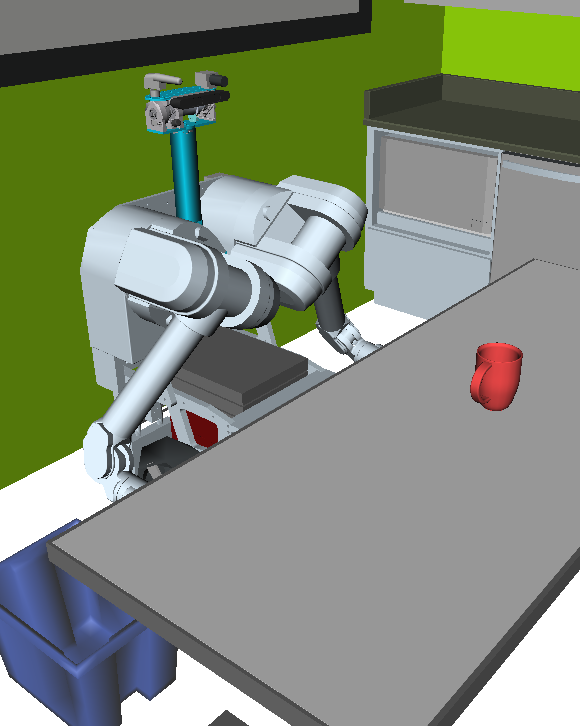
\includegraphics[width=\columnwidth]{figs/testherb-a.png}
\caption{Start config}
\end{subfigure}
\begin{subfigure}[t]{0.19\linewidth}
\centering
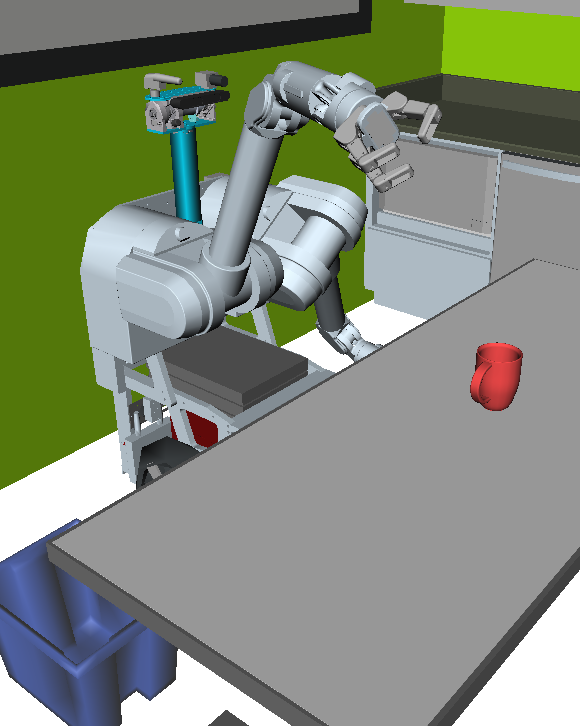
\includegraphics[width=\columnwidth]{figs/testherb-b.png}
\caption{Part 1 in $X_1$}
\end{subfigure}
\begin{subfigure}[t]{0.19\linewidth}
\centering
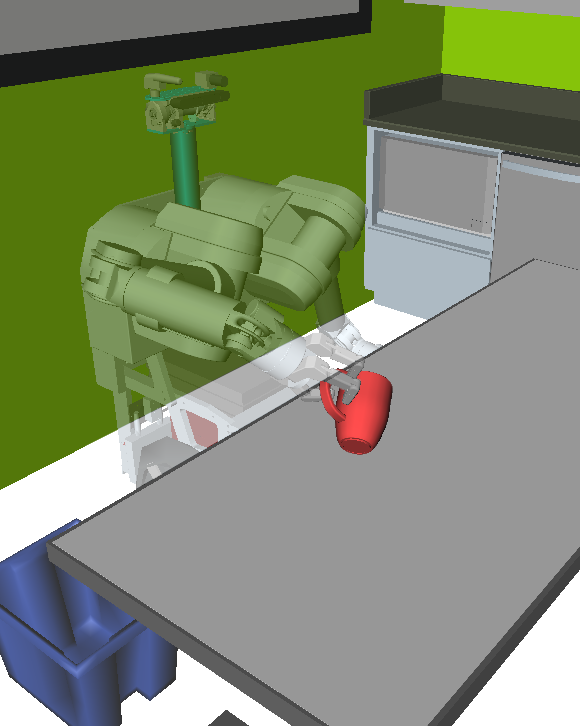
\includegraphics[width=\columnwidth]{figs/testherb-c.png}
\caption{Part 2 in $X_2$}
\end{subfigure}
\begin{subfigure}[t]{0.19\linewidth}
\centering
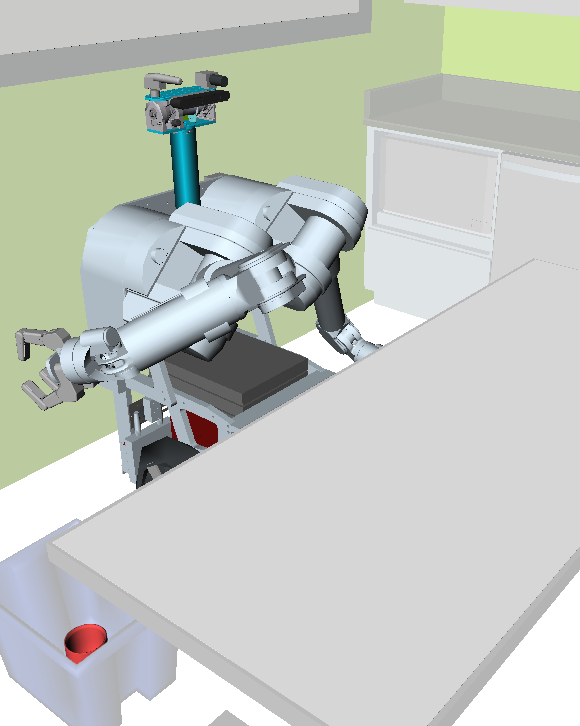
\includegraphics[width=\columnwidth]{figs/testherb-d.png}
\caption{Part 3 in $X_3$}
\end{subfigure}
\begin{subfigure}[t]{0.19\linewidth}
\centering
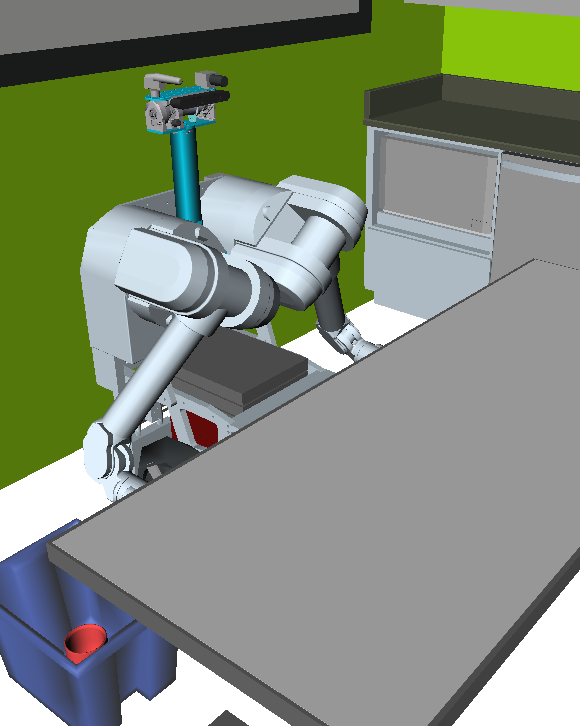
\includegraphics[width=\columnwidth]{figs/testherb-e.png}
\caption{End config}
\end{subfigure}

\vspace{0.1in}

   \begin{subfigure}[b]{4.0in}
      \begin{center}
      \includegraphics{build/intro-subprob-cspace}
      \end{center}
      \caption{Plan sequences
         within distinct free $\mathcal{C}$-subsets
         from the problem above.}
   \end{subfigure}%
   \quad%
   \begin{subfigure}[b]{2.0in}
      \begin{center}
      \includegraphics{build/intro-subprob-axis}
      \end{center}
      \caption{Single vs. Multi Query Planners}
   \end{subfigure}
   \caption{\textsc{Herb} plans for a simple manipulation task
      to grasp, transfer, and drop a mug from a table into a bin
      before returning to an end configuration.
      Each sub-problem requires a path in a distinct free subset of
      configuration space;
      our approach enables partial reuse between these parts.}
   \label{fig:intro-multi-part}
\end{center}
\end{widepage}
\end{figure}
}

While planning cost is a significant component
in resource-constrained human-scale problems,
manipulation tasks exhibit a structure
which makes it difficult to apply fast planning approaches.
In particular,
they are inherently composed of multiple distinct sub-problems,
each of which 
must be validated a different subset of configuration space,
which makes traditional multi-query planners impractical.
For example, see the manipulation task in
Figure~\ref{fig:intro-multi-part}.

We solve this in two ways.
First, in Chapter~\ref{chap:multi-set},
we introduce the \emph{multi-set planning problem}.
We show that while the valid subsets are different for each part,
they are related in a structured way.
In fact, we show how lots of different prior ideas for planner
efficiency are unified by this formalism.

Second, Chapter~\ref{chap:multi-set-prm}
uses the multi-set formalism as a planning cost model
for the E$^8$-PRM.
The resulting algorithm,
the Multi-Set PRM,
uses propositional logic to represent the multi-set structure
algorithmically.
%We show how we can use incremental graph search approaches
%to make it super fast.

\textbf{Challenge 3: Task Robustness Requires Long-Horizon Plans.}

Not only does the structure of manipulation tasks
impede planner reuse between sub-problems,
but it also necessitates long-horizon plans to ensure robustness.
For example,
consider sequentially planning for the task in
Figure~\ref{fig:intro-multi-part}.
The interfaces between these parts lie on continuous manifolds.
A choice made by an early planning part
-- e.g. what arm configuration or object grasp to use --
often renders a subsequent part either difficult to plan,
costly to execute, or impossible altogether.

Many planners are designed to take as input start and/or goal sets.
We might hope that we can delegate each task sub-problem to
separate such planner instances,
and provide each with specifications for their corresponding
root sets.
However,
a customary planning request takes an \emph{any-to-any} form
(i.e. from \emph{any} start to \emph{any} goal configuration).
Clearly, without coordination,
the juxtaposed paths will not be continuous.

We mitigate this in two parts.
First, we introduce the \emph{Comprehensive Multi-Root} (CMR) planner
objective (Chapter~\ref{chap:cmr}).
In constrast to the traditional any-to-any objective,
CMR encourages a planner to discover paths between multiple pairs of
roots.

Second,
we introduce the \textsc{Proteus} task planner
(Chapter~\ref{chap:task-planning})
which restricts each sub-problem to a limited set of samples
for each interface manifold
by performing root sampling
and coordinates between sub-planners.

\textbf{Applications and Experiments.}

We give a bunch of examples of this framework
for different robots.
For example, I really want to talk about robots idly
hypothesizing worlds.


\textbf{Summary of Proposed Work.}

See Chapter~\ref{chap:proposed}
for a summary and timeline of proposed work.


{
\setlength{\offsetpage}{0.75in}
\begin{figure}[t]
\begin{widepage}
\begin{center}
\begin{tikzpicture}

% axes
\draw[->,thick] (0,0) -- (0,8); 
\draw[->,thick] (0,0) -- (12,0);
\node[rotate=90,align=center] at (-1.0,4)
   {Challenge 1:\\Task Efficiency};
\node[align=center] at (6,-1.6)
   {Challenge 2:\\Sub-Problem Structure};

% y tics
\draw (-0.2,1) -- (0.2,1);
\node[rotate=90,align=center] at (-0.64,1)
   {considers\\[-0.04in]execution cost};
\draw (-0.2,7) -- (0.2,7);
\node[rotate=90,align=center] at (-0.8,7)
   {considers\\[-0.04in]planning and\\[-0.04in]execution cost};

% x tics
\draw (2,-0.2) -- (2,0.2);
\node[align=center] at (2,-0.5) {no reuse};
\draw (6,-0.2) -- (6,0.2);
\node[align=center] at (6,-0.5) {two-set reuse};
\draw (10,-0.2) -- (10,0.2);
\node[align=center] at (10,-0.5) {full reuse};

% algorithms
\node[draw,ellipse,align=center] at (2,1)
   {Lazy PRM \cite{bohlin2000lazyprm}};

\node[draw,ellipse,align=center] at (6,1)
   {\cite{leven2000changing}, \cite{kallman2004dynamicroadmaps},
   \cite{jaillet2004dynamicprm}};

\node[draw,ellipse,align=center] at (2,7)
   {E$^8$-PRM\\(Chapter~\ref{chap:e8})};

\node[draw,ellipse,align=center] at (10,7)
   {Multi-Set PRM\\(Chapter~\ref{chap:multi-set-prm})};

\end{tikzpicture}
\caption{Graphical outline of $\mathcal{C}$-space planners.
   \cdnote{Work in progress. I don't really like this as it is.}}
\label{fig:graphical-outline}
\end{center}
\end{widepage}
\end{figure}
}

%\begin{figure}
%\begin{widepage}
%   \centering
%   \begin{subfigure}[b]{0.24\textwidth}
%      \begin{center}
%      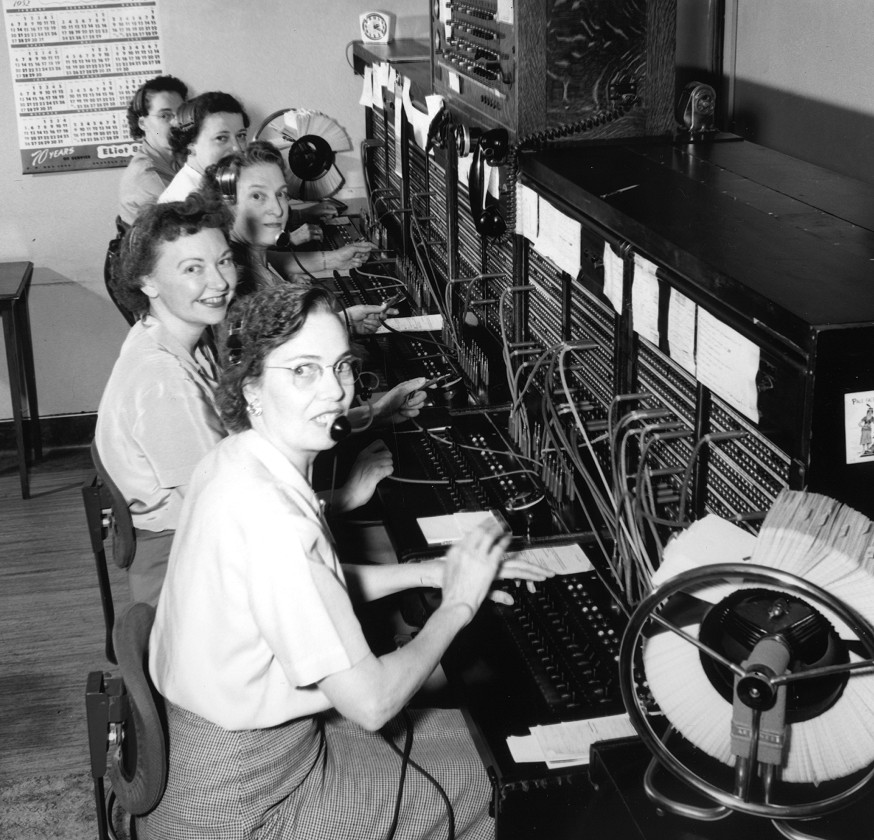
\includegraphics[width=\textwidth]{figs/switchboard.jpg}
%      
%      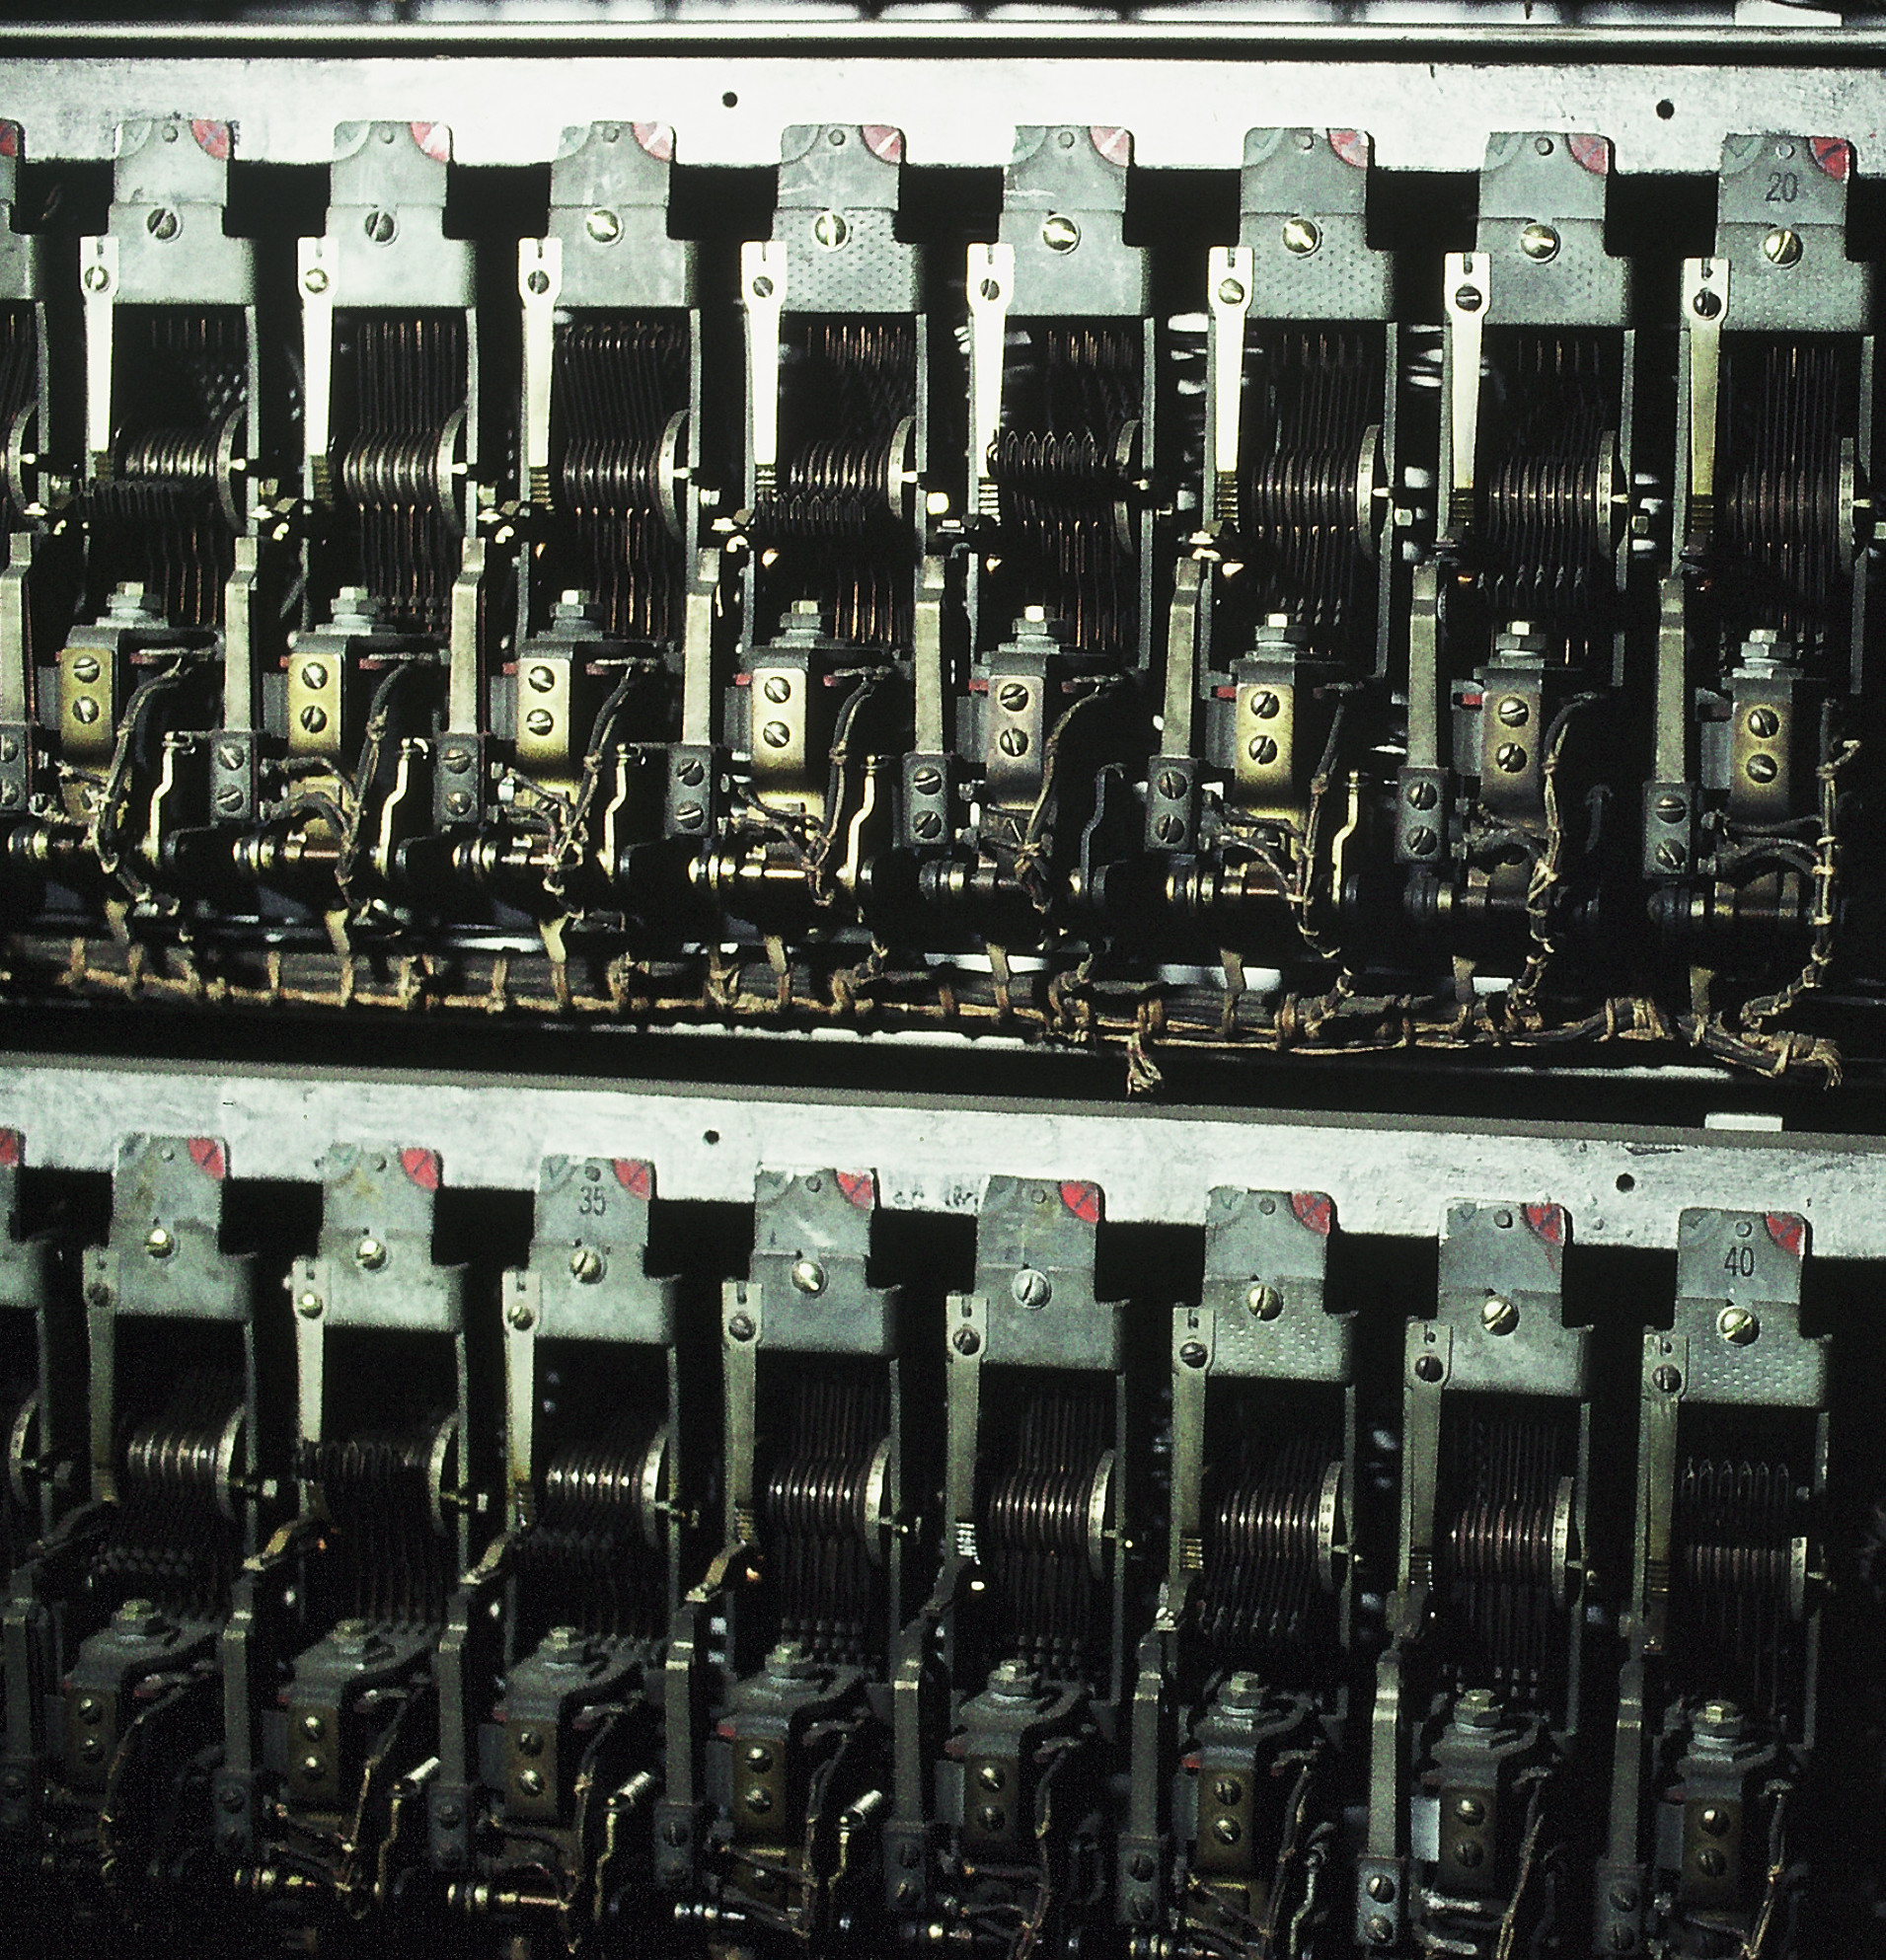
\includegraphics[width=\textwidth]{figs/mech-switches.jpg}
%      \end{center}
%      \caption{Something}
%   \end{subfigure}
%   \begin{subfigure}[b]{0.24\textwidth}
%      \begin{center}
%      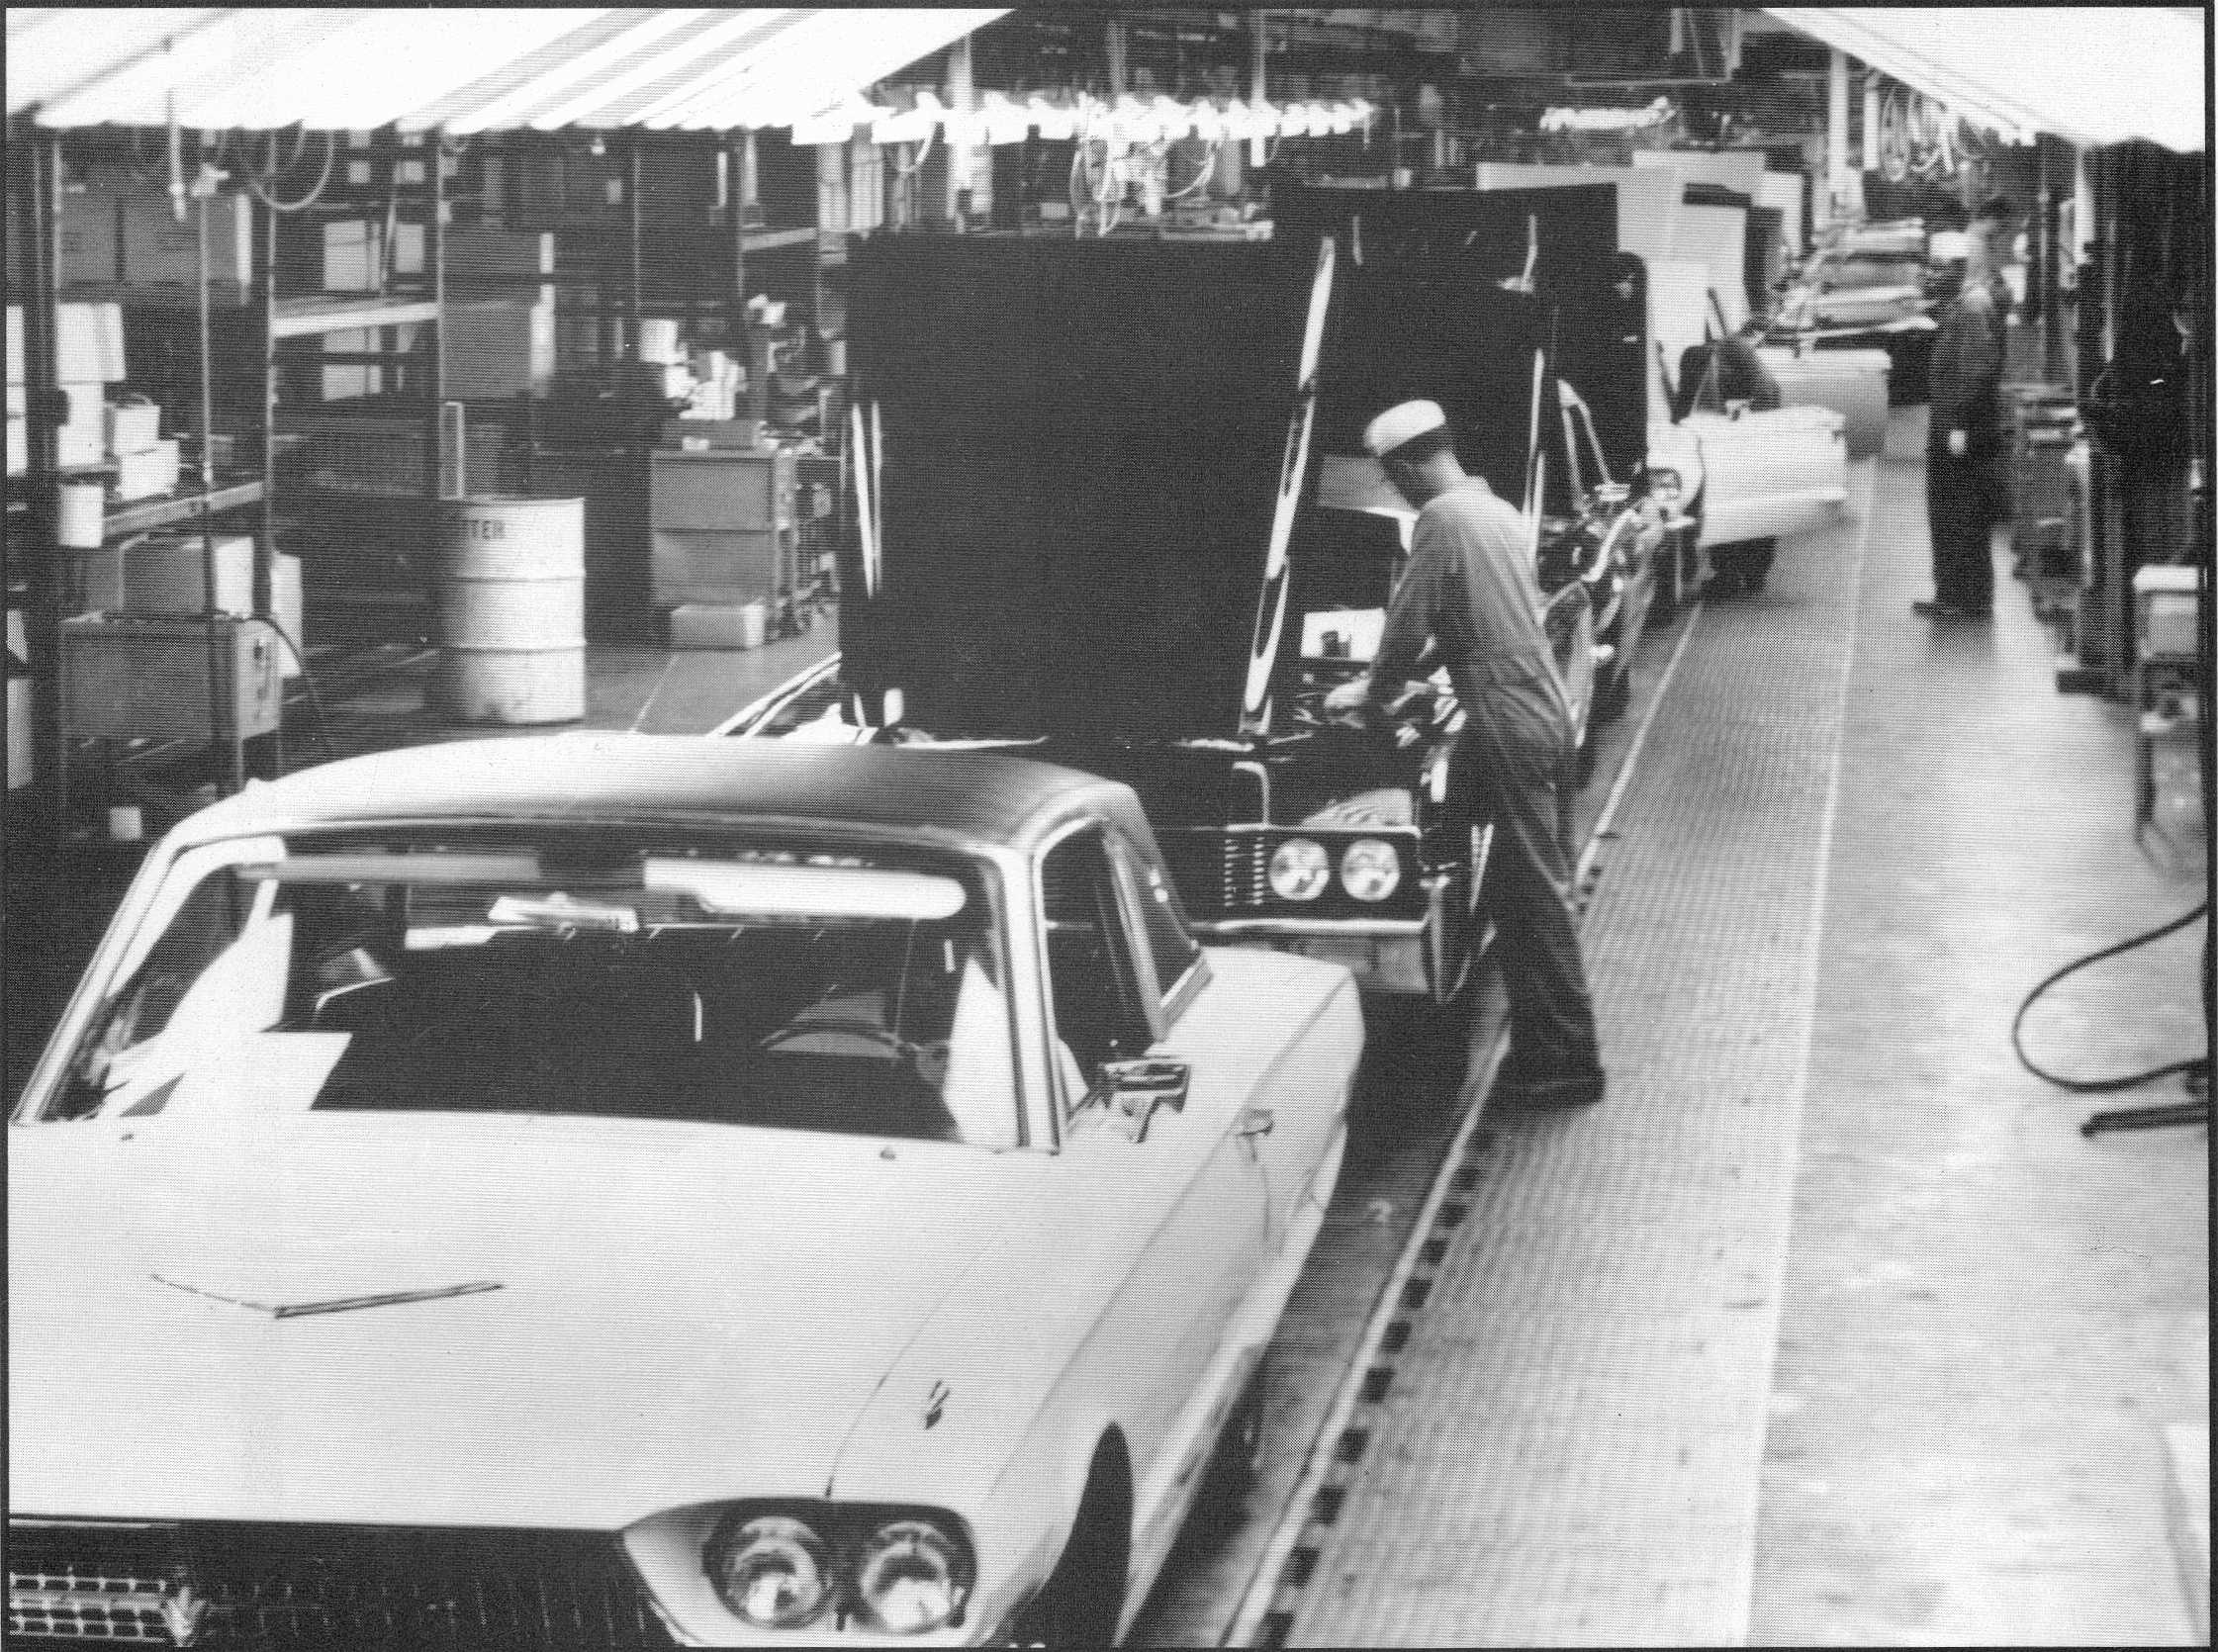
\includegraphics[width=\textwidth]{figs/assembly-line.jpg}
%      
%      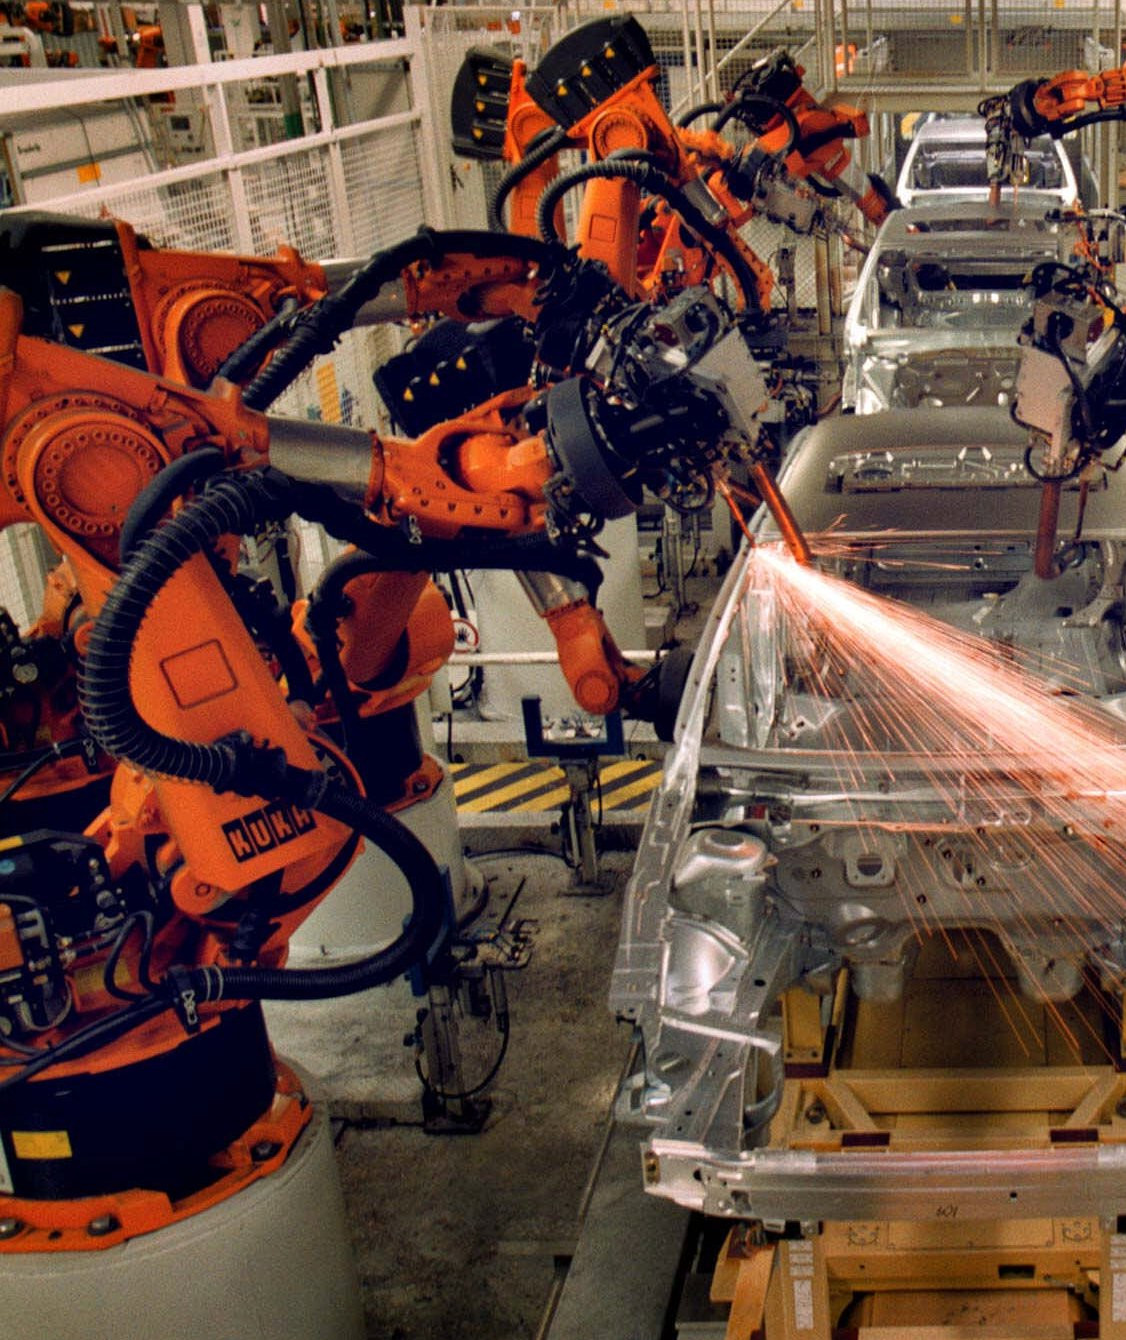
\includegraphics[width=\textwidth]{figs/car-robots.jpg}
%      \end{center}
%      \caption{Something}
%   \end{subfigure}
%   \begin{subfigure}[b]{0.24\textwidth}
%      \begin{center}
%      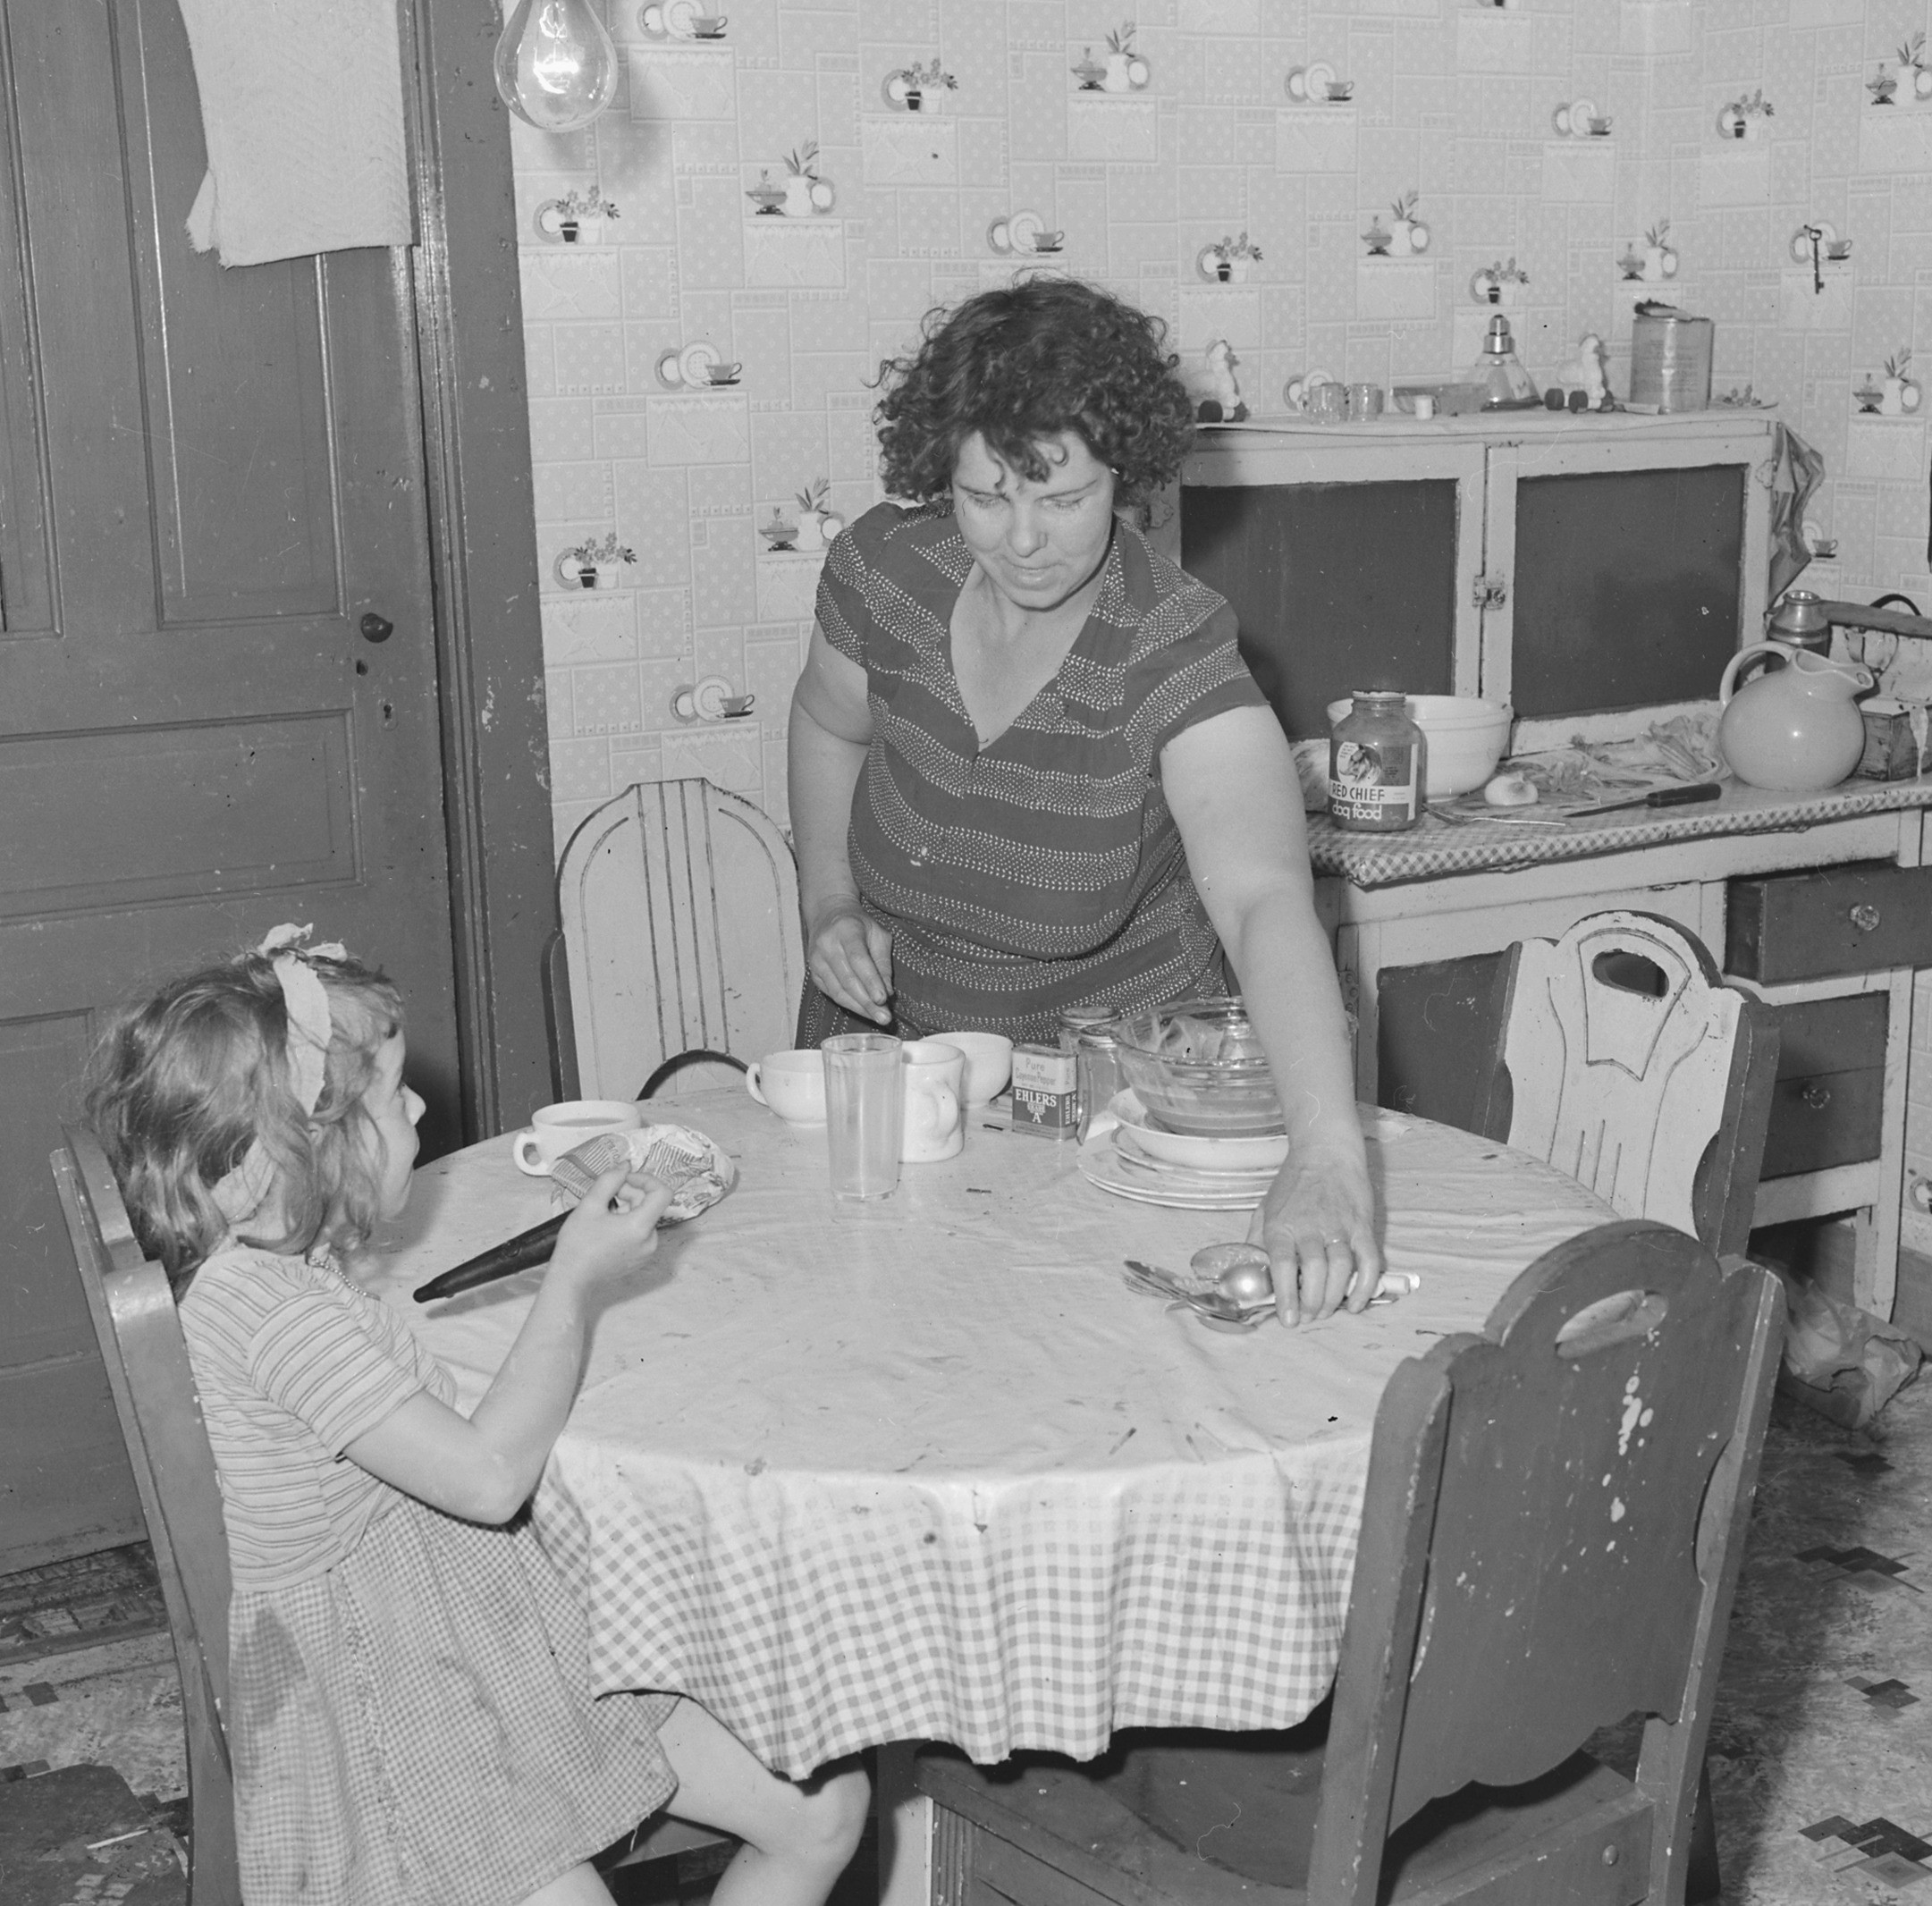
\includegraphics[width=\textwidth]{figs/table-clearing.jpg}
%      
%      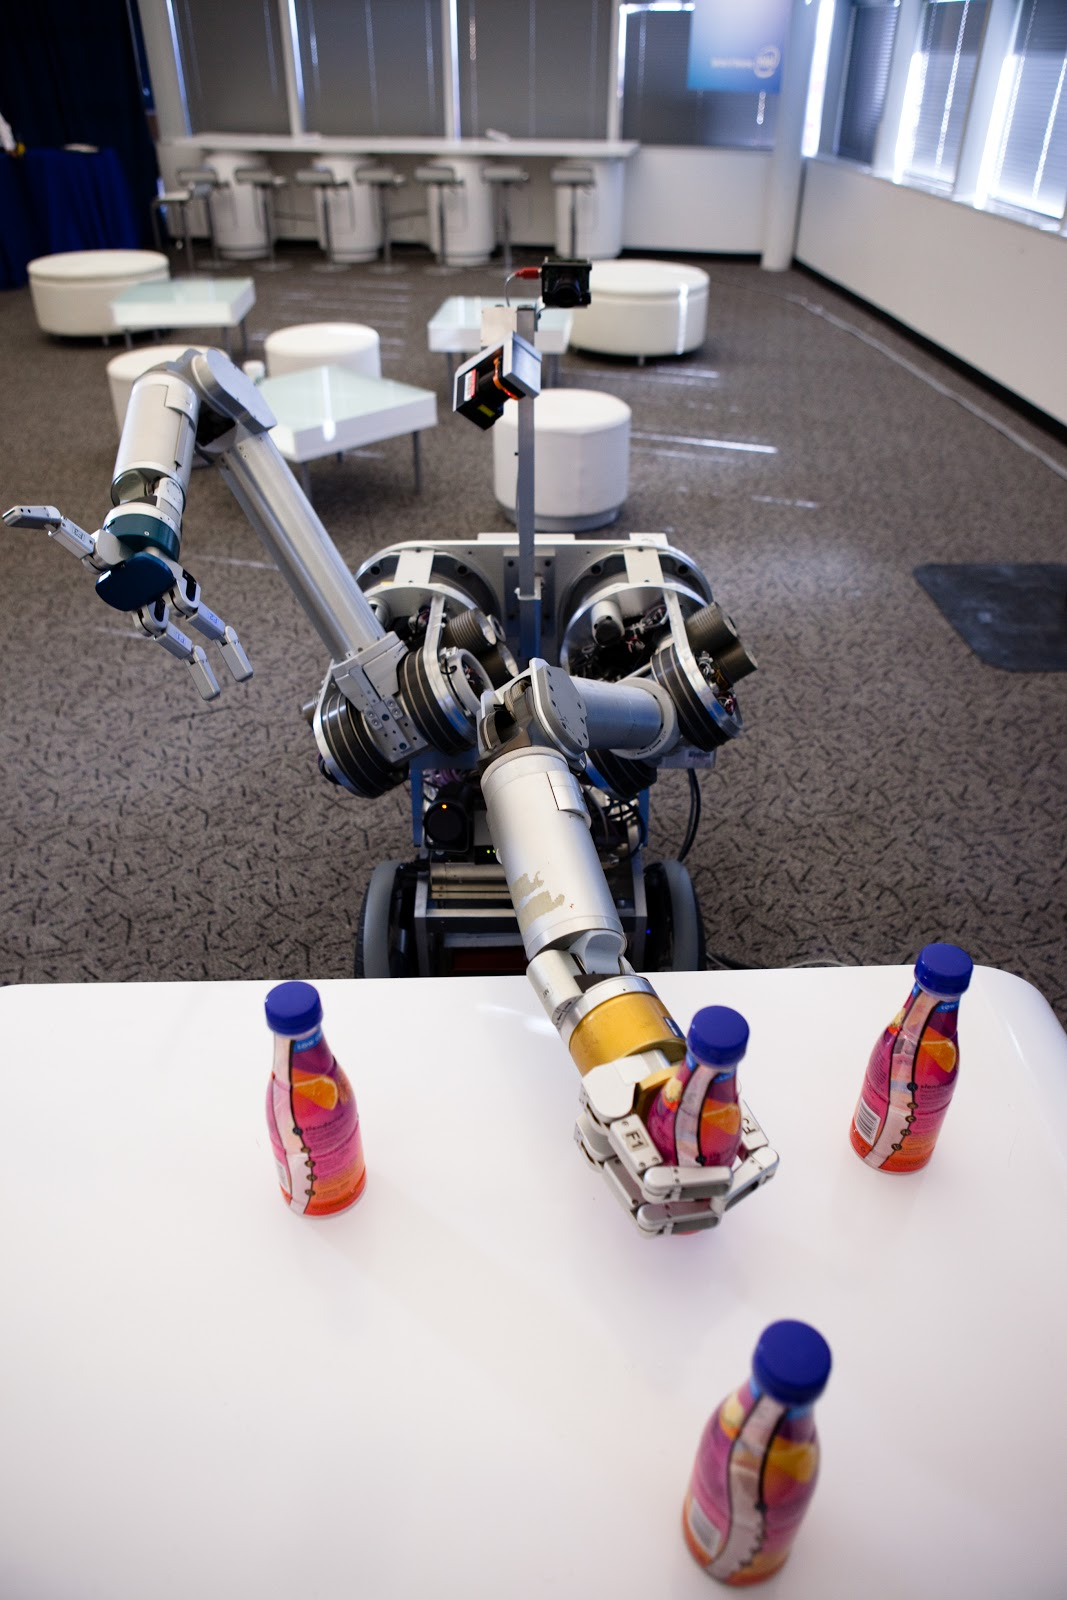
\includegraphics[height=2in]{figs/herb-fuze.jpg}
%      \end{center}
%      \caption{HERB Robot}
%   \end{subfigure}
%   \begin{subfigure}[b]{0.24\textwidth}
%      \begin{center}
%      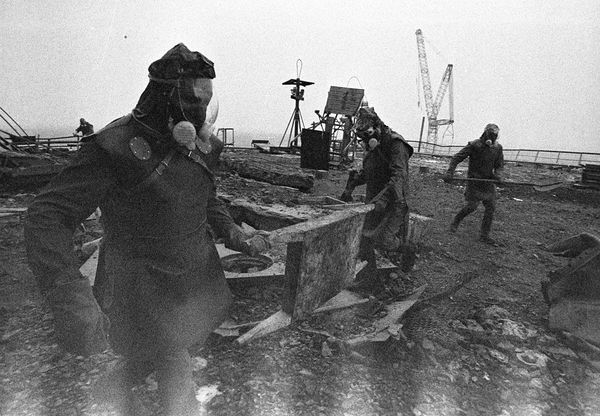
\includegraphics[width=\textwidth]{figs/chernobyl.jpg}
%      
%      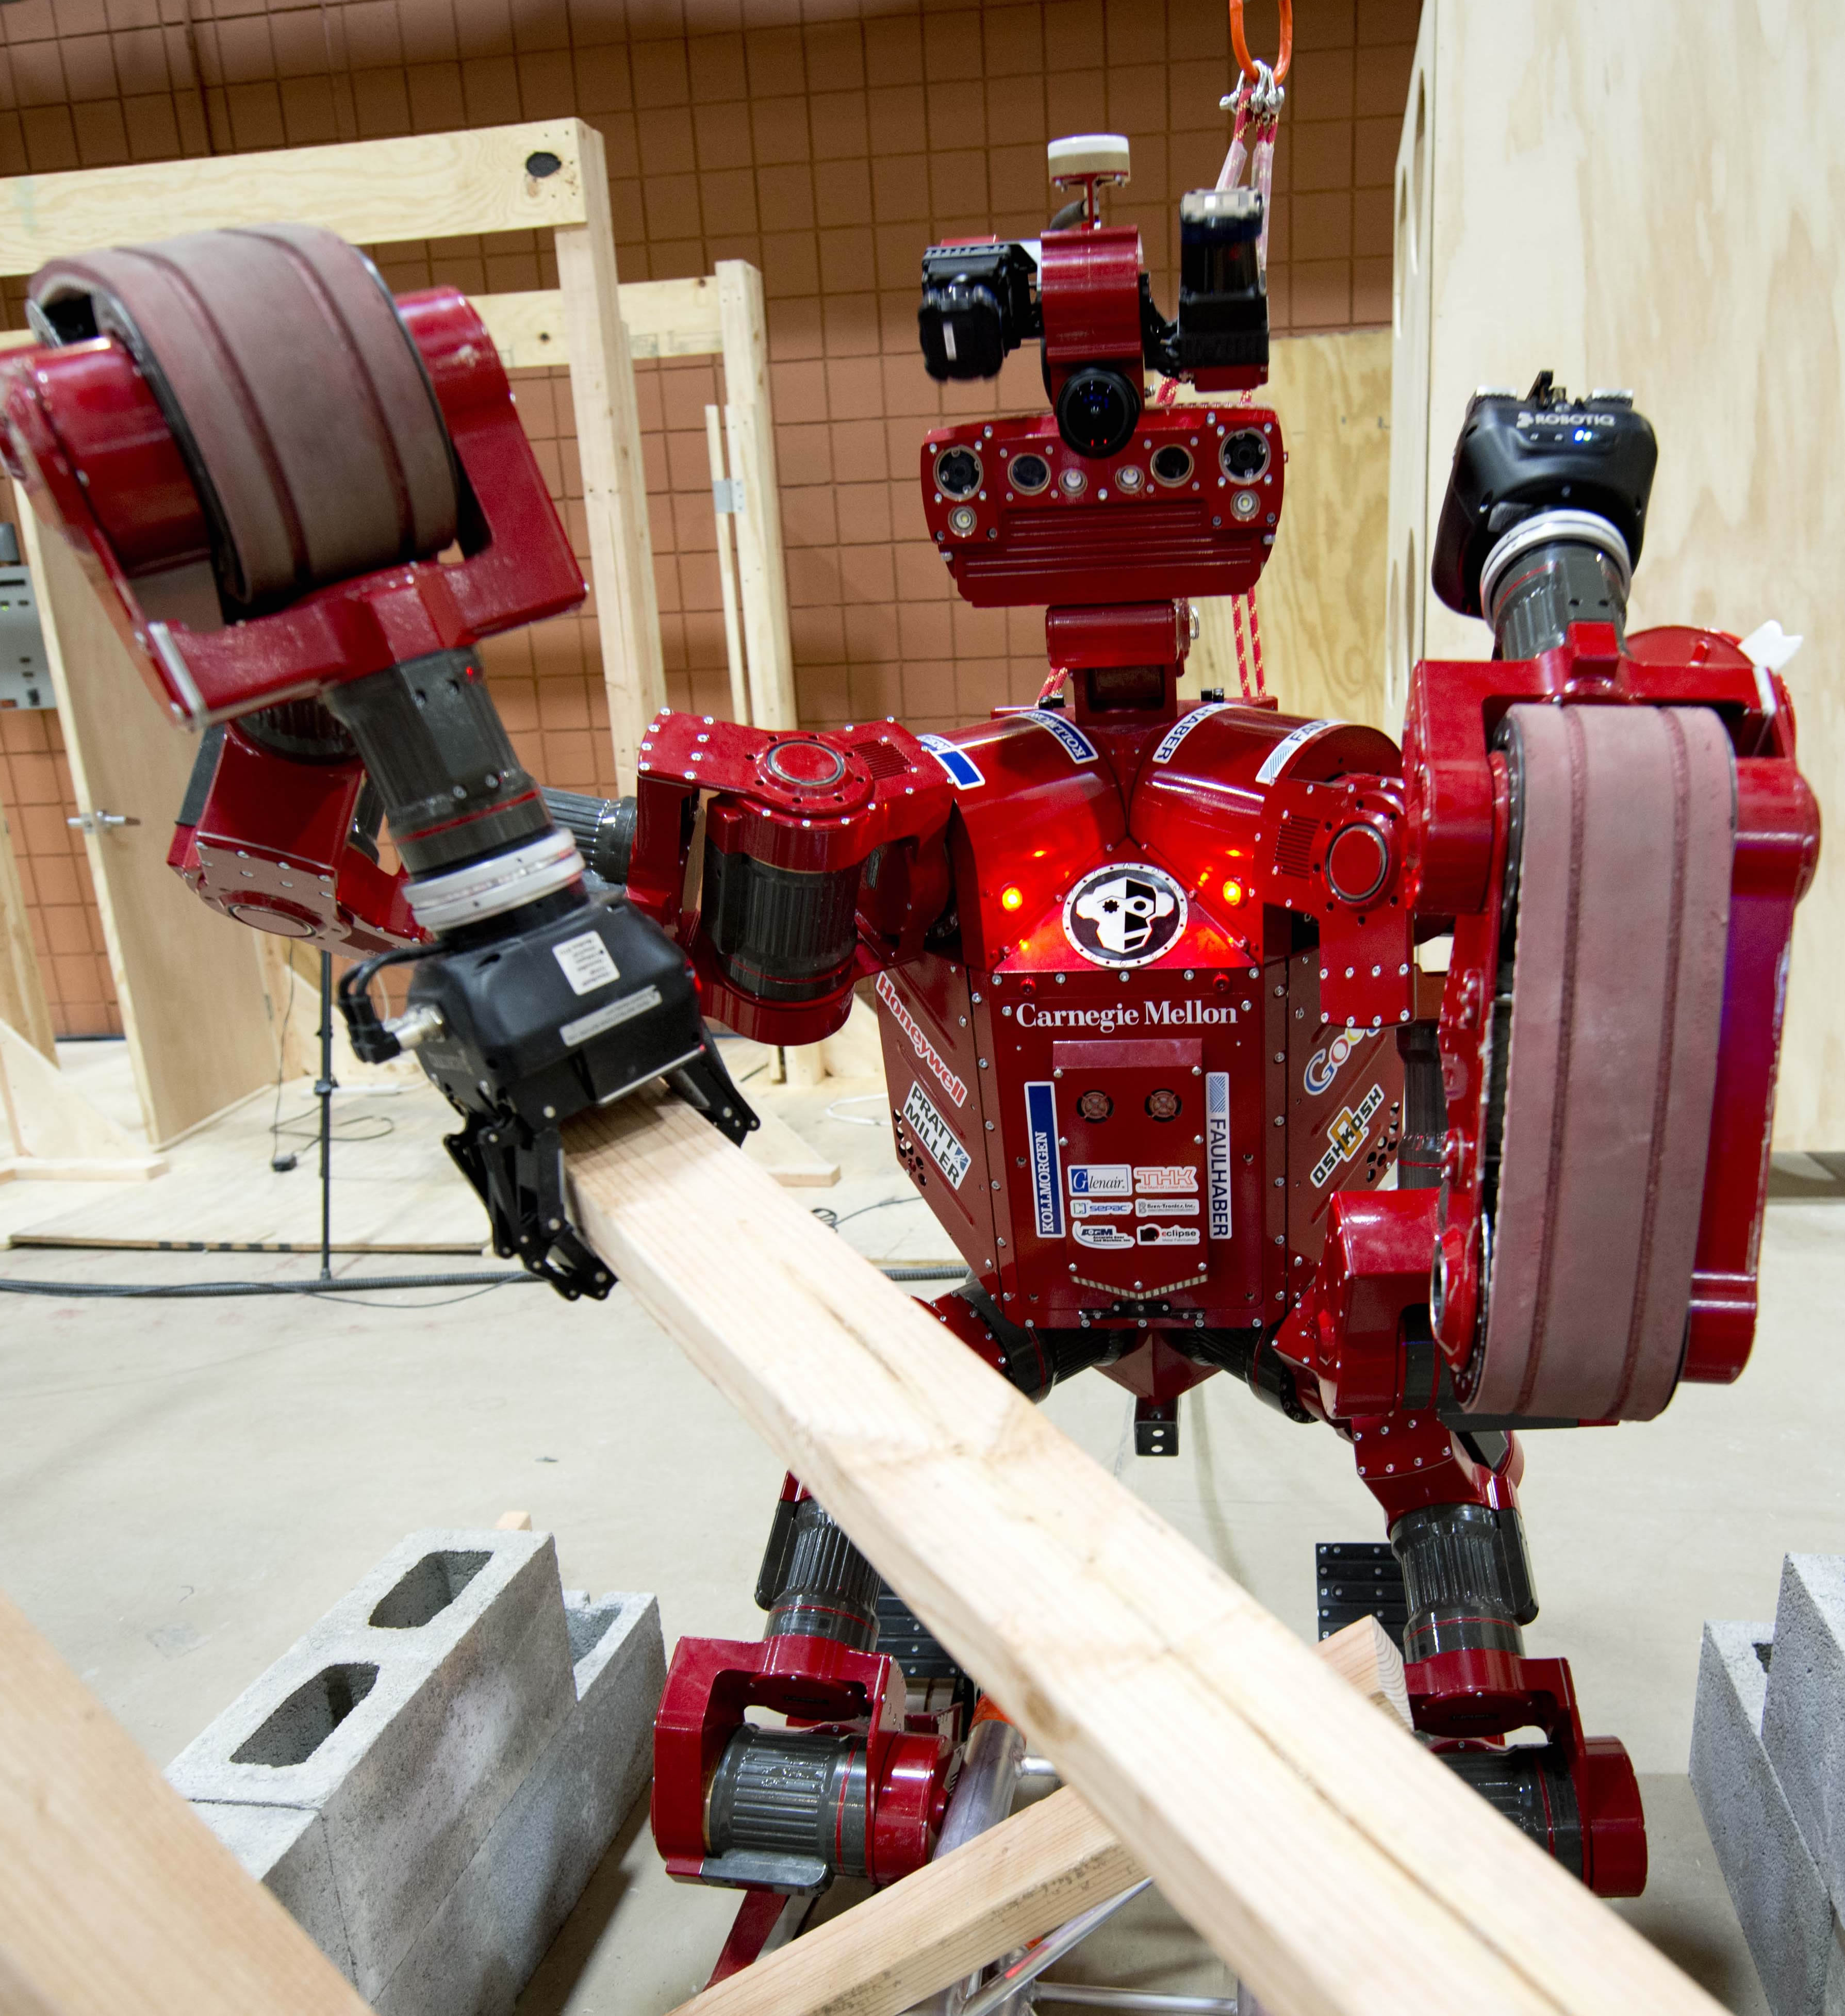
\includegraphics[height=2in]{figs/chimp-debris.jpg}
%      \end{center}
%      \caption{CHIMP Robot}
%   \end{subfigure}
%   \caption{Manipulation problems.}
%\end{widepage}
%\end{figure}
